% =============================================================================
% Lecture 08: Regularization — LASSO, Ridge, Elastic Net
% BSAD 8310: Business Forecasting | University of Nebraska at Omaha
% =============================================================================
\documentclass[aspectratio=169, 10pt]{beamer}
% =============================================================================
% header.tex — BSAD 8310: Business Forecasting
% University of Nebraska at Omaha
% Beamer theme: UNO-branded, clean, professional
% =============================================================================

% ----------------------------- BEAMER THEME ----------------------------------
\usetheme{default}
\useinnertheme{rectangles}

% ----------------------------- UNO COLOR PALETTE -----------------------------
\definecolor{unoblue}{HTML}{005CA9}
\definecolor{unored}{HTML}{E41C38}
\definecolor{unogray}{HTML}{525252}
\definecolor{unogreen}{HTML}{15803d}
\definecolor{unolightblue}{HTML}{E8F0FA}
\definecolor{unolightred}{HTML}{FDECEA}
\definecolor{unolightgreen}{HTML}{F0FAF4}
\definecolor{unowhite}{HTML}{FFFFFF}

% Apply UNO colors to Beamer structure
\setbeamercolor{structure}{fg=unoblue}
\setbeamercolor{palette primary}{bg=unoblue, fg=white}
\setbeamercolor{palette secondary}{bg=unoblue!80!black, fg=white}
\setbeamercolor{palette tertiary}{bg=unoblue!60!black, fg=white}
\setbeamercolor{frametitle}{bg=unoblue, fg=white}
\setbeamercolor{frametitle right}{bg=unoblue!80!black}
\setbeamercolor{title}{fg=unoblue}
\setbeamercolor{subtitle}{fg=unogray}
\setbeamercolor{author in head/foot}{bg=unoblue, fg=white}
\setbeamercolor{title in head/foot}{bg=unoblue!80, fg=white}
\setbeamercolor{date in head/foot}{bg=unoblue!60, fg=white}
\setbeamercolor{page number in head/foot}{bg=unoblue!60, fg=white}
\setbeamercolor{block title}{bg=unoblue, fg=white}
\setbeamercolor{block body}{bg=unolightblue}
\setbeamercolor{block title alerted}{bg=unored, fg=white}
\setbeamercolor{block body alerted}{bg=unolightred}
\setbeamercolor{block title example}{bg=unogreen, fg=white}
\setbeamercolor{block body example}{bg=unolightgreen}
\setbeamercolor{itemize item}{fg=unoblue}
\setbeamercolor{itemize subitem}{fg=unored}
\setbeamercolor{enumerate item}{fg=unoblue}
\setbeamercolor{enumerate subitem}{fg=unored}
\setbeamercolor{alerted text}{fg=unored}

% ----------------------------- FONTS -----------------------------------------
\usefonttheme{professionalfonts}
\usefonttheme[onlymath]{serif}       % serif math; sans-serif text
\setbeamerfont{frametitle}{size=\large, series=\bfseries}
\setbeamerfont{title}{size=\LARGE, series=\bfseries}
\setbeamerfont{subtitle}{size=\large}
\setbeamerfont{block title}{size=\normalsize, series=\bfseries}
\setbeamerfont{footline}{size=\tiny}

% ----------------------------- LAYOUT ----------------------------------------
\setbeamersize{text margin left=0.5cm, text margin right=0.5cm}
\setbeamertemplate{navigation symbols}{}   % remove navigation buttons
\setbeamertemplate{itemize items}[circle]
\setbeamertemplate{enumerate items}[default]

% Custom footline: [Course] [Title] [Page/Total]
\setbeamertemplate{footline}{%
  \leavevmode%
  \hbox{%
    \begin{beamercolorbox}[wd=.33\paperwidth, ht=2.5ex, dp=1ex, left, leftskip=4pt]
      {author in head/foot}%
      \usebeamerfont{author in head/foot}\insertshortauthor
    \end{beamercolorbox}%
    \begin{beamercolorbox}[wd=.34\paperwidth, ht=2.5ex, dp=1ex, center]
      {title in head/foot}%
      \usebeamerfont{title in head/foot}\insertshorttitle
    \end{beamercolorbox}%
    \begin{beamercolorbox}[wd=.33\paperwidth, ht=2.5ex, dp=1ex, right, rightskip=4pt]
      {date in head/foot}%
      \usebeamerfont{date in head/foot}%
      \insertframenumber{} / \inserttotalframenumber
    \end{beamercolorbox}%
  }%
  \vskip0pt%
}

% Frametitle with thin accent line
\setbeamertemplate{frametitle}{%
  \vskip0.1cm
  \insertframetitle
  \vskip0.05cm
  \color{unored}\rule{\textwidth}{0.5pt}
}

% Title page
\setbeamertemplate{title page}{%
  \vfill
  \begin{center}
    {\color{unoblue}\rule{\textwidth}{2pt}}\\[0.3cm]
    {\usebeamerfont{title}\usebeamercolor[fg]{title}\inserttitle}\\[0.2cm]
    {\usebeamerfont{subtitle}\usebeamercolor[fg]{subtitle}\insertsubtitle}\\[0.3cm]
    {\color{unored}\rule{\textwidth}{0.5pt}}\\[0.4cm]
    {\small\insertauthor}\\[0.1cm]
    {\small\insertinstitute}\\[0.1cm]
    {\small\insertdate}
  \end{center}
  \vfill
}

% ----------------------------- PACKAGES --------------------------------------

% Math
\usepackage{amsmath}
\usepackage{amssymb}
\usepackage{mathtools}
\usepackage{bm}                    % bold math symbols

% Graphics & color
\usepackage{graphicx}
\usepackage{xcolor}
\usepackage{tikz}
\usetikzlibrary{arrows.meta, positioning, shapes, fit, backgrounds, calc}
\usepackage{pgfplots}
\pgfplotsset{compat=1.18}

% Tables
\usepackage{booktabs}
\usepackage{array}
\usepackage{multirow}
\usepackage{tabularx}

% Typography
\usepackage{microtype}
\usepackage{url}
\usepackage{hyperref}
\hypersetup{colorlinks=true, linkcolor=unoblue, urlcolor=unoblue, citecolor=unogray}

% Code listings (no shell-escape required)
\usepackage{listings}
\lstset{
  language=Python,
  basicstyle=\ttfamily\footnotesize,
  keywordstyle=\color{unoblue}\bfseries,
  stringstyle=\color{unogreen},
  commentstyle=\color{unogray}\itshape,
  numberstyle=\tiny\color{unogray},
  breaklines=true,
  showstringspaces=false,
  frame=single,
  rulecolor=\color{unogray!40},
  backgroundcolor=\color{unogray!5},
  xleftmargin=0.5em,
  xrightmargin=0.5em,
}

% Bibliography
\usepackage[backend=bibtex, style=authoryear, maxcitenames=2]{biblatex}
\addbibresource{../Bibliography_base.bib}

% Colored text helpers
\usepackage{tcolorbox}
\tcbuselibrary{skins, breakable, listingsutf8}

% ----------------------------- CUSTOM ENVIRONMENTS ---------------------------

% keybox: UNO-blue background — for key results, formulas, takeaways
\newtcolorbox{keybox}{
  enhanced,
  colback=unoblue,
  colframe=unoblue!80!black,
  coltitle=white,
  coltext=white,
  fonttitle=\bfseries,
  boxrule=0pt,
  arc=3pt,
  left=4pt, right=4pt, top=3pt, bottom=3pt,
}

% definitionbox: blue left-rule with title — for formal definitions
\newtcolorbox{definitionbox}[1]{
  enhanced,
  title={#1},
  colback=unolightblue,
  colframe=unoblue,
  coltitle=unoblue,
  fonttitle=\bfseries,
  boxrule=0pt,
  leftrule=3pt,
  arc=0pt,
  left=4pt, right=4pt, top=3pt, bottom=3pt,
}

% warningbox: red-accent — for pitfalls, assumption violations, common errors
\newtcolorbox{warningbox}{
  enhanced,
  colback=unolightred,
  colframe=unored,
  coltitle=white,
  fonttitle=\bfseries,
  boxrule=0pt,
  leftrule=3pt,
  arc=0pt,
  left=4pt, right=4pt, top=3pt, bottom=3pt,
}

% examplebox: green-accent with title — for worked examples, business applications
\newtcolorbox{examplebox}[1]{
  enhanced,
  title={#1},
  colback=unolightgreen,
  colframe=unogreen,
  coltitle=unogreen,
  fonttitle=\bfseries,
  boxrule=0pt,
  leftrule=3pt,
  arc=0pt,
  left=4pt, right=4pt, top=3pt, bottom=3pt,
}

% ----------------------------- MATH SHORTCUTS --------------------------------
\newcommand{\E}{\mathbb{E}}
\newcommand{\Var}{\operatorname{Var}}
\newcommand{\Cov}{\operatorname{Cov}}
\newcommand{\Corr}{\operatorname{Corr}}
\newcommand{\MSE}{\operatorname{MSE}}
\newcommand{\RMSE}{\operatorname{RMSE}}
\newcommand{\MAE}{\operatorname{MAE}}
\newcommand{\MASE}{\operatorname{MASE}}
\newcommand{\yhat}{\hat{y}}
\newcommand{\bhat}{\hat{\beta}}
\newcommand{\eps}{\varepsilon}
\newcommand{\given}{\,|\,}

% ----------------------------- SLIDE HELPERS ---------------------------------
% Section title slide (call at start of each section)
\newcommand{\sectionslide}[2]{%
  \begin{frame}
    \vfill
    \begin{center}
      {\color{unoblue}\rule{0.6\textwidth}{2pt}}\\[0.4cm]
      {\Large\bfseries\color{unoblue} #1}\\[0.2cm]
      {\normalsize\color{unogray} #2}\\[0.4cm]
      {\color{unored}\rule{0.6\textwidth}{1pt}}
    \end{center}
    \vfill
  \end{frame}
}

% Muted text
\newcommand{\muted}[1]{{\color{unogray}#1}}

% Key term
\newcommand{\key}[1]{{\color{unoblue}\textbf{#1}}}

% Positive / negative annotations
\newcommand{\pos}[1]{{\color{unogreen}#1}}
\newcommand{\negc}[1]{{\color{unored}#1}}


\title{Lecture 08: Regularization}
\subtitle{LASSO, Ridge, and Elastic Net for Forecasting}
\author{BSAD 8310: Business Forecasting}
\institute{University of Nebraska at Omaha}
\date{Spring 2026}

% =============================================================================
\begin{document}
% =============================================================================

\begin{frame}
  \titlepage
\end{frame}

% -----------------------------------------------------------------------------
\begin{frame}{Lecture Outline}
% -----------------------------------------------------------------------------
  \tableofcontents
\end{frame}

% =============================================================================
\section{Motivation: Why Regularization?}
% =============================================================================

\sectionslide{Motivation: Why Regularization?}{%
  OLS breaks down when predictors are many, correlated, or $p \to n$.\\
  Regularization trades a little bias for large variance reduction.}

\begin{frame}{Section Overview}
  \textbf{The problem:} OLS breaks down when predictors are many, correlated,
  or when $p$ approaches $n$. Regularization adds a penalty that trades a
  little bias for a large variance reduction.
\end{frame}

% -----------------------------------------------------------------------------
\begin{frame}{OLS Instability with Many Predictors}
% -----------------------------------------------------------------------------
  \textbf{Recall OLS:} $\hat{\bm{\beta}} = (\mathbf{X}^\top\mathbf{X})^{-1}\mathbf{X}^\top\mathbf{y}$

  \medskip
  \textbf{Three failure modes in forecasting:}
  \begin{enumerate}
    \item \textbf{Near-multicollinearity} — $\mathbf{X}^\top\mathbf{X}$ is nearly singular;
          small data perturbations flip sign and magnitude of $\hat{\bm{\beta}}$
    \item \textbf{High dimensionality} — with $p$ lags + rolling features + calendar dummies,
          $p$ can approach or exceed $n$
    \item \textbf{Overfitting} — OLS minimizes in-sample RSS exactly;
          generalization to new periods is poor
  \end{enumerate}

  \medskip
  \begin{examplebox}{RSXFS Feature Matrix}
    With 12 lags + 3 rolling windows + 12 month dummies = 27 predictors on
    $n \approx 300$ monthly obs.\ Small by ML standards, but already
    enough for OLS instability with correlated lag features.
  \end{examplebox}
\end{frame}

% -----------------------------------------------------------------------------
\begin{frame}{The Bias--Variance View}
% -----------------------------------------------------------------------------
  \begin{columns}[T]
    \begin{column}{0.54\textwidth}
      \textbf{OLS is unbiased but high-variance:}
      \[
        \mathbb{E}[\hat{\bm{\beta}}_{\mathrm{OLS}}] = \bm{\beta}
        \quad \text{but} \quad
        \mathrm{Var}(\hat{\bm{\beta}}_{\mathrm{OLS}}) \text{ large}
      \]

      \textbf{Regularized estimator accepts bias:}
      \[
        \mathbb{E}[\hat{\bm{\beta}}_{\lambda}] \neq \bm{\beta}
        \quad \text{but} \quad
        \mathrm{Var}(\hat{\bm{\beta}}_{\lambda}) \text{ smaller}
      \]

      \medskip
      Net effect: \textbf{lower MSE} in finite samples when
      variance reduction exceeds the squared-bias increase.
    \end{column}
    \begin{column}{0.42\textwidth}
      \begin{keybox}
        \textbf{Bias--Variance Decomposition}\\[4pt]
        $\mathrm{MSE} = \mathrm{Bias}^2 + \mathrm{Var} + \sigma^2$\\[4pt]
        Regularization shifts the tradeoff leftward along the \emph{model complexity} axis.
      \end{keybox}
    \end{column}
  \end{columns}
\end{frame}

% -----------------------------------------------------------------------------
\begin{frame}{Penalized Regression: General Form}
% -----------------------------------------------------------------------------
  All penalised regression methods solve:
  \[
    \hat{\bm{\beta}}_\lambda
    = \arg\min_{\bm{\beta}}
      \underbrace{\|\mathbf{y} - \mathbf{X}\bm{\beta}\|_2^2}_{\text{fit (RSS)}}
      + \lambda \cdot \underbrace{P(\bm{\beta})}_{\text{penalty}}
  \]

  \medskip
  \begin{center}
    \footnotesize
    \begin{tabular}{lll}
      \toprule
      \textbf{Method} & \textbf{Penalty} $P(\bm{\beta})$ & \textbf{Key property} \\
      \midrule
      Ridge      & $\|\bm{\beta}\|_2^2 = \sum_j \beta_j^2$              & Shrinks, never zeros \\
      LASSO      & $\|\bm{\beta}\|_1 = \sum_j |\beta_j|$                & Shrinks + selects \\
      Elastic Net & $\alpha\|\bm{\beta}\|_1 + (1-\alpha)\|\bm{\beta}\|_2^2$ & Both \\
      \bottomrule
    \end{tabular}
  \end{center}

  \medskip
  \muted{\footnotesize\itshape
    $\lambda \geq 0$ controls penalty strength; $\lambda=0$ recovers OLS.
    $\lambda \to \infty$ shrinks $\hat{\bm{\beta}} \to \bm{0}$.
    The tuning of $\lambda$ (and $\alpha$ for Elastic Net) is covered in Section~6.}
\end{frame}

% =============================================================================
\section{Ridge Regression (L2)}
% =============================================================================

\sectionslide{Ridge Regression (L2)}{%
  Shrinks all coefficients toward zero; handles multicollinearity with a closed-form solution.}

\begin{frame}{Section Overview}
  \textbf{Ridge regression} adds an L2 penalty that shrinks all coefficients
  toward zero but never sets them exactly to zero. It has an analytical
  solution and handles multicollinearity well.
\end{frame}

% -----------------------------------------------------------------------------
\begin{frame}{Ridge: Objective and Solution}
% -----------------------------------------------------------------------------
  \begin{definitionbox}{Ridge Regression}
    \[
      \hat{\bm{\beta}}^{\mathrm{R}}_\lambda
      = \arg\min_{\bm{\beta}} \|\mathbf{y} - \mathbf{X}\bm{\beta}\|_2^2
        + \lambda \|\bm{\beta}\|_2^2
    \]
    \textbf{Analytical solution:}
    \[
      \hat{\bm{\beta}}^{\mathrm{R}}_\lambda
      = \left(\mathbf{X}^\top\mathbf{X} + \lambda \mathbf{I}\right)^{-1}
        \mathbf{X}^\top\mathbf{y}
    \]
  \end{definitionbox}

  \medskip
  \textbf{Why does this fix near-singularity?}
  \begin{itemize}
    \item $\mathbf{X}^\top\mathbf{X}$ may be near-singular (smallest eigenvalue $\approx 0$)
    \item Adding $\lambda\mathbf{I}$ shifts all eigenvalues up by $\lambda$:
          matrix becomes safely invertible \parencite{HoerlKennard1970}
    \item Coefficients shrink by factor $d_j^2 / (d_j^2 + \lambda)$ along
          each principal direction $j$ (SVD interpretation)
  \end{itemize}
\end{frame}

% -----------------------------------------------------------------------------
\begin{frame}{Ridge: Constraint Set Geometry}
% -----------------------------------------------------------------------------
  \begin{columns}[T]
    \begin{column}{0.48\textwidth}
      \textbf{Equivalent constrained form:}
      \[
        \min_{\bm{\beta}} \|\mathbf{y}-\mathbf{X}\bm{\beta}\|_2^2
        \quad \text{s.t.}\ \|\bm{\beta}\|_2^2 \leq t
      \]

      \medskip
      The Ridge constraint set is a \textbf{sphere} (circle in 2D).
      The OLS solution is usually outside; the Ridge solution is the
      point where the RSS ellipses first touch the sphere.

      \medskip
      \begin{warningbox}
        Coefficients are \textbf{never exactly zero} — the sphere has no corners.
        Ridge does \emph{not} perform variable selection.
      \end{warningbox}
    \end{column}
    \begin{column}{0.48\textwidth}
      % Ridge geometry: circle constraint
      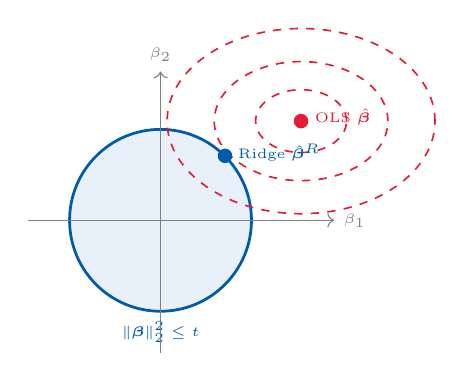
\begin{tikzpicture}[scale=1.05]
        % Constraint circle
        \draw[fill=unolightblue, draw=unoblue, line width=1pt] (0,0) circle (1.1cm);
        \node[font=\tiny, color=unoblue] at (0,-1.35) {$\|\bm{\beta}\|_2^2 \leq t$};
        % OLS solution
        \fill[unored] (1.7, 1.2) circle (2.5pt);
        \node[font=\tiny, right, color=unored] at (1.75,1.25) {OLS $\hat{\bm{\beta}}$};
        % RSS ellipses (3 concentric)
        \draw[unored, dashed, line width=0.6pt] (1.7,1.2) ellipse (0.55cm and 0.38cm);
        \draw[unored, dashed, line width=0.6pt] (1.7,1.2) ellipse (1.05cm and 0.72cm);
        \draw[unored, dashed, line width=0.6pt] (1.7,1.2) ellipse (1.62cm and 1.12cm);
        % Ridge solution (on circle boundary)
        \fill[unoblue] (0.78, 0.78) circle (2.5pt);
        \node[font=\tiny, right, color=unoblue] at (0.82, 0.82) {Ridge $\hat{\bm{\beta}}^R$};
        % Axes
        \draw[->, gray, thin] (-1.6,0)--(2.1,0) node[right,font=\tiny]{$\beta_1$};
        \draw[->, gray, thin] (0,-1.6)--(0,1.8) node[above,font=\tiny]{$\beta_2$};
      \end{tikzpicture}
    \end{column}
  \end{columns}
\end{frame}

% -----------------------------------------------------------------------------
\begin{frame}{Ridge: Coefficient Path}
% -----------------------------------------------------------------------------
  As $\lambda$ increases from 0 to $\infty$, all coefficients shrink
  \emph{smoothly} toward zero:

  \begin{center}
  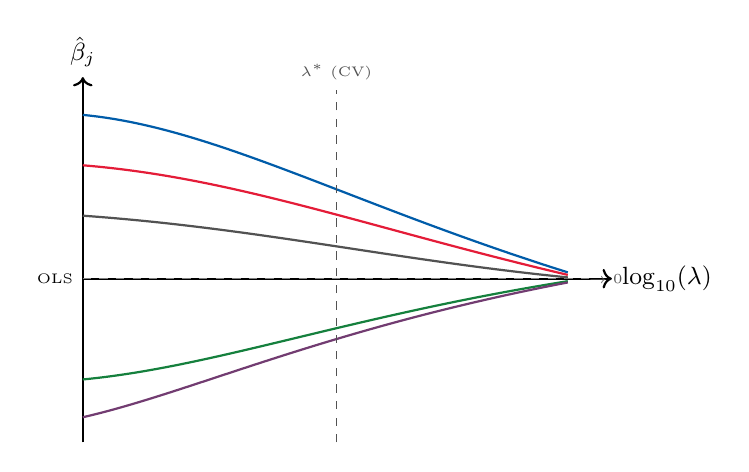
\begin{tikzpicture}[xscale=2.8, yscale=1.6]
    % Axes
    \draw[->, thick] (0,0) -- (2.4,0) node[right, font=\small]{$\log_{10}(\lambda)$};
    \draw[->, thick] (0,-1.3) -- (0,1.6) node[above, font=\small]{$\hat{\beta}_j$};
    \draw[dashed, gray] (0,0) -- (2.3,0);
    % 5 coefficient paths (hardcoded smooth curves shrinking to 0)
    \draw[unoblue, thick]
      (0, 1.3) .. controls (0.6,1.2) and (1.2,0.6) .. (2.2, 0.05);
    \draw[unored, thick]
      (0, 0.9) .. controls (0.7,0.8) and (1.3,0.4) .. (2.2, 0.03);
    \draw[unogreen, thick]
      (0, -0.8) .. controls (0.6,-0.7) and (1.2,-0.3) .. (2.2, -0.02);
    \draw[unogray, thick]
      (0, 0.5) .. controls (0.8,0.4) and (1.4,0.15) .. (2.2, 0.01);
    \draw[unoblue!50!unored, thick]
      (0, -1.1) .. controls (0.5,-0.9) and (1.1,-0.4) .. (2.2, -0.03);
    % OLS label at left
    \node[font=\tiny, left] at (0, 0) {OLS};
    % Zero label
    \node[font=\tiny, right, unogray] at (2.25, 0) {$\to 0$};
    % Lambda star marker
    \draw[dashed, unogray] (1.15, -1.3) -- (1.15, 1.5)
      node[above, font=\tiny, unogray]{$\lambda^*$ (CV)};
  \end{tikzpicture}
  \end{center}

  \muted{\footnotesize\itshape Socratic: if two predictors are perfectly correlated,
  what does Ridge do to their coefficients? What does LASSO do? (Answered in the next section.)}
\end{frame}

% -----------------------------------------------------------------------------
\begin{frame}{Ridge: Key Properties Summary}
% -----------------------------------------------------------------------------
  \begin{columns}[T]
    \begin{column}{0.48\textwidth}
      \textbf{Strengths:}
      \begin{itemize}
        \item Closed-form solution — fast computation
        \item Handles multicollinearity: correlated predictors get
              \emph{equal} shrinkage (spread out penalty)
        \item Continuous, stable in $\lambda$
        \item Works when $p > n$
      \end{itemize}
    \end{column}
    \begin{column}{0.48\textwidth}
      \textbf{Limitations:}
      \begin{itemize}
        \item \textbf{No variable selection} — all $p$ predictors remain in model
        \item Interpretation harder with many near-zero (but non-zero) coefficients
        \item Requires \textbf{standardized} predictors (or use sklearn
              \texttt{Pipeline} with \texttt{StandardScaler})
      \end{itemize}
    \end{column}
  \end{columns}

  \medskip
  \begin{keybox}
    \textbf{When to use Ridge:} when you believe \emph{all} predictors contribute
    a little (dense signal), or when predictors are highly correlated groups.
  \end{keybox}
\end{frame}

% =============================================================================
\section{LASSO Regression (L1)}
% =============================================================================

\sectionslide{LASSO Regression (L1)}{%
  Shrinks \emph{and} selects: L1 penalty sets irrelevant coefficients to exactly zero \parencite{Tibshirani1996}.}

\begin{frame}{Section Overview}
  \textbf{LASSO} (Least Absolute Shrinkage and Selection Operator) uses an L1
  penalty that both shrinks coefficients \emph{and} sets some exactly to zero.
  It performs automatic variable selection \parencite{Tibshirani1996}.
\end{frame}

% -----------------------------------------------------------------------------
\begin{frame}{LASSO: Objective and Sparsity}
% -----------------------------------------------------------------------------
  \begin{definitionbox}{LASSO Regression}
    \[
      \hat{\bm{\beta}}^{\mathrm{L}}_\lambda
      = \arg\min_{\bm{\beta}} \|\mathbf{y} - \mathbf{X}\bm{\beta}\|_2^2
        + \lambda \|\bm{\beta}\|_1
    \]
    \[
      \|\bm{\beta}\|_1 = \sum_{j=1}^{p} |\beta_j|
    \]
  \end{definitionbox}

  \smallskip
  \textbf{No closed form} — solved by \textbf{coordinate descent}:
  update one $\beta_j$ at a time, applying \emph{soft-thresholding}:
  \[
    \hat{\beta}_j \leftarrow
    \mathrm{sign}(z_j)\,\max\!\left(|z_j| - \tfrac{\lambda}{2},\, 0\right)
  \]
  where $z_j$ is the partial-residual inner product for predictor $j$.
  When $|z_j| \leq \lambda/2$, coefficient is set \textbf{exactly to zero}.

  \smallskip
  {\footnotesize\textbf{Example} ($\lambda=2$, threshold $=1$):
  $z_j = 1.8 \Rightarrow \hat{\beta}_j = +0.8$;\quad
  $z_j = 0.7 \Rightarrow \hat{\beta}_j = 0$ \muted{(zeroed out)}.}
\end{frame}

% -----------------------------------------------------------------------------
\begin{frame}{LASSO: Constraint Set Geometry}
% -----------------------------------------------------------------------------
  \begin{columns}[T]
    \begin{column}{0.48\textwidth}
      \textbf{Equivalent constrained form:}
      \[
        \min_{\bm{\beta}} \|\mathbf{y}-\mathbf{X}\bm{\beta}\|_2^2
        \quad \text{s.t.}\ \|\bm{\beta}\|_1 \leq t
      \]

      \medskip
      The LASSO constraint set is a \textbf{diamond} (rotated square in 2D).
      The RSS ellipses typically first touch the diamond at a \textbf{corner},
      where one or more $\beta_j = 0$ exactly.

      \medskip
      \begin{keybox}
        The corners of the $\ell_1$ ball are the source of sparsity.
        In $p$ dimensions: exponentially many corners at coordinate axes.
      \end{keybox}
    \end{column}
    \begin{column}{0.48\textwidth}
      % LASSO geometry: diamond constraint
      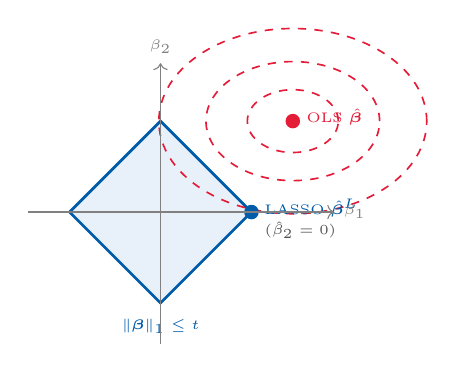
\begin{tikzpicture}[scale=1.05]
        % Diamond constraint set
        \fill[unolightblue] (0,1.1) -- (1.1,0) -- (0,-1.1) -- (-1.1,0) -- cycle;
        \draw[unoblue, line width=1pt] (0,1.1) -- (1.1,0) -- (0,-1.1) -- (-1.1,0) -- cycle;
        \node[font=\tiny, color=unoblue] at (0,-1.38) {$\|\bm{\beta}\|_1 \leq t$};
        % OLS solution
        \fill[unored] (1.6, 1.1) circle (2.5pt);
        \node[font=\tiny, right, color=unored] at (1.65,1.15) {OLS $\hat{\bm{\beta}}$};
        % RSS ellipses
        \draw[unored, dashed, line width=0.6pt] (1.6,1.1) ellipse (0.55cm and 0.38cm);
        \draw[unored, dashed, line width=0.6pt] (1.6,1.1) ellipse (1.05cm and 0.72cm);
        \draw[unored, dashed, line width=0.6pt] (1.6,1.1) ellipse (1.62cm and 1.12cm);
        % LASSO solution at corner (beta_2 = 0)
        \fill[unoblue] (1.1, 0) circle (2.5pt);
        \node[font=\tiny, right, color=unoblue] at (1.14, 0.05)
          {LASSO $\hat{\bm{\beta}}^L$};
        \node[font=\tiny, right, color=unogray] at (1.14, -0.22)
          {($\hat{\beta}_2 = 0$)};
        % Axes
        \draw[->, gray, thin] (-1.6,0)--(2.1,0) node[right,font=\tiny]{$\beta_1$};
        \draw[->, gray, thin] (0,-1.6)--(0,1.8) node[above,font=\tiny]{$\beta_2$};
      \end{tikzpicture}
    \end{column}
  \end{columns}
\end{frame}

% -----------------------------------------------------------------------------
\begin{frame}{LASSO: Coefficient Path}
% -----------------------------------------------------------------------------
  As $\lambda$ increases, LASSO coefficients shrink and hit zero at different $\lambda$ values:

  \begin{center}
  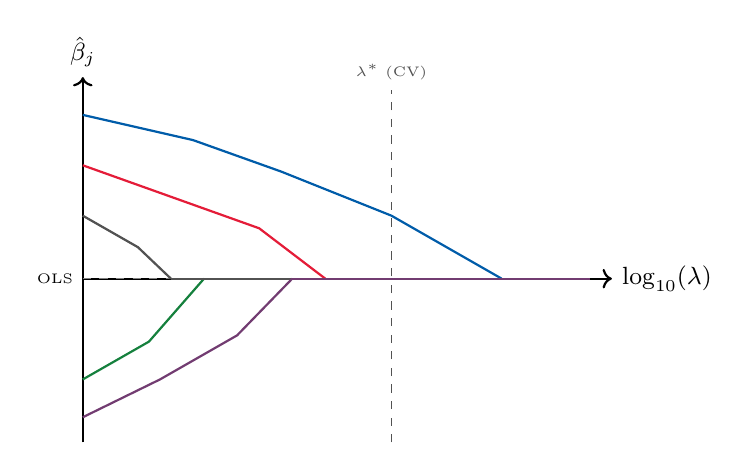
\begin{tikzpicture}[xscale=2.8, yscale=1.6]
    % Axes
    \draw[->, thick] (0,0) -- (2.4,0) node[right, font=\small]{$\log_{10}(\lambda)$};
    \draw[->, thick] (0,-1.3) -- (0,1.6) node[above, font=\small]{$\hat{\beta}_j$};
    \draw[dashed, gray] (0,0) -- (2.3,0);
    % Coefficient paths (LASSO: piecewise linear, hit 0 at different lambda)
    % beta_1: large positive, last to zero out
    \draw[unoblue, thick]
      (0, 1.3) -- (0.5,1.1) -- (0.9,0.85) -- (1.4,0.5) -- (1.9,0);
    \draw[unoblue, thick] (1.9,0) -- (2.3,0);
    % beta_2: moderate positive
    \draw[unored, thick]
      (0, 0.9) -- (0.4,0.65) -- (0.8,0.4) -- (1.1,0);
    \draw[unored, thick] (1.1,0) -- (2.3,0);
    % beta_3: negative, zeroed early
    \draw[unogreen, thick]
      (0, -0.8) -- (0.3,-0.5) -- (0.55,0);
    \draw[unogreen, thick] (0.55,0) -- (2.3,0);
    % beta_4: small positive, zeroed early
    \draw[unogray, thick]
      (0, 0.5) -- (0.25,0.25) -- (0.4,0);
    \draw[unogray, thick] (0.4,0) -- (2.3,0);
    % beta_5: moderate negative
    \draw[unoblue!50!unored, thick]
      (0, -1.1) -- (0.35,-0.8) -- (0.7,-0.45) -- (0.95,0);
    \draw[unoblue!50!unored, thick] (0.95,0) -- (2.3,0);
    % OLS label
    \node[font=\tiny, left] at (0, 0) {OLS};
    % Lambda star marker
    \draw[dashed, unogray] (1.4, -1.3) -- (1.4, 1.5)
      node[above, font=\tiny, unogray]{$\lambda^*$ (CV)};
  \end{tikzpicture}
  \end{center}

  \muted{\footnotesize\itshape Note the kinks (piecewise-linear path) — a consequence
  of coordinate descent and the L1 geometry. Ridge paths are smooth curves.}
\end{frame}

% -----------------------------------------------------------------------------
\begin{frame}{LASSO: Properties and Limitations}
% -----------------------------------------------------------------------------
  \begin{columns}[T]
    \begin{column}{0.48\textwidth}
      \textbf{Strengths:}
      \begin{itemize}
        \item \textbf{Automatic variable selection} — irrelevant lags zeroed out
        \item Interpretable: small active set survives
        \item Works when $p \gg n$
        \item Coefficient path is a diagnostic: shows which features enter first
      \end{itemize}
    \end{column}
    \begin{column}{0.48\textwidth}
      \textbf{Limitations:}
      \begin{itemize}
        \item \textbf{Grouped predictors problem} — among correlated features,
              LASSO picks one arbitrarily and zeros others
        \item Non-unique solution when $p > n$
        \item Slower than Ridge (no closed form)
        \item Sensitive to feature scaling (must standardize)
      \end{itemize}
    \end{column}
  \end{columns}

  \medskip
  \begin{examplebox}{RSXFS Application}
    With 12 monthly lags, LASSO typically retains lags 1, 3, 12 and zeros
    lags 4–11 — consistent with retail seasonality and recency effects.
    Rolling-window features may or may not survive depending on $\lambda^*$.
  \end{examplebox}
\end{frame}

% =============================================================================
\section{Elastic Net}
% =============================================================================

\sectionslide{Elastic Net}{%
  Combines L1 and L2 penalties: sparsity from LASSO, grouped selection from Ridge \parencite{ZouHastie2005}.}

\begin{frame}{Section Overview}
  \textbf{Elastic Net} combines L1 and L2 penalties to get the best of both:
  sparsity from LASSO and grouped selection from Ridge. It uses two
  hyperparameters: $\lambda$ (overall strength) and $\alpha$ (mix ratio)
  \parencite{ZouHastie2005}.

  \smallskip
  \muted{\footnotesize\itshape Note: $\alpha$ here is the L1/L2 mixing parameter ---
  distinct from the level-smoothing $\alpha$ in ETS (Lecture~03)
  and the ECM speed-of-adjustment $\alpha$ in Lecture~05.}
\end{frame}

% -----------------------------------------------------------------------------
\begin{frame}{Elastic Net: Objective and Geometry}
% -----------------------------------------------------------------------------
  \begin{definitionbox}{Elastic Net}
    \[
      \hat{\bm{\beta}}^{\mathrm{EN}}_{\lambda,\alpha}
      = \arg\min_{\bm{\beta}} \|\mathbf{y} - \mathbf{X}\bm{\beta}\|_2^2
        + \lambda \left[\alpha \|\bm{\beta}\|_1
          + (1-\alpha)\|\bm{\beta}\|_2^2\right]
    \]
    \begin{itemize}
      \item $\alpha = 1$: pure LASSO
      \item $\alpha = 0$: pure Ridge
      \item $0 < \alpha < 1$: Elastic Net (interpolates between them)
    \end{itemize}
  \end{definitionbox}

  \medskip
  \textbf{Grouped selection property:} when predictors are correlated,
  Elastic Net tends to include or exclude them as a group — unlike LASSO
  which arbitrarily picks one.

  \medskip
  \begin{columns}[T]
    \begin{column}{0.5\textwidth}
      \textbf{Two hyperparameters to tune:}
      \begin{itemize}
        \item $\lambda$ (penalty magnitude): grid search via CV
        \item $\alpha$ (mix): try $\{0.1, 0.5, 0.9\}$ or use \texttt{ElasticNetCV}
      \end{itemize}
    \end{column}
    \begin{column}{0.46\textwidth}
      \begin{warningbox}
        Tuning both $\lambda$ and $\alpha$ simultaneously is expensive.
        Start with fixed $\alpha=0.5$ and tune $\lambda$ only.
      \end{warningbox}
    \end{column}
  \end{columns}
\end{frame}

% -----------------------------------------------------------------------------
\begin{frame}{Ridge vs.\ LASSO vs.\ Elastic Net: Decision Guide}
% -----------------------------------------------------------------------------
  \begin{center}
  \footnotesize
  \begin{tabular}{p{2.8cm}p{3.0cm}p{3.0cm}p{3.0cm}}
    \toprule
    \textbf{Situation} & \textbf{Ridge} & \textbf{LASSO} & \textbf{Elastic Net} \\
    \midrule
    Dense signal (all $\beta_j \neq 0$)
      & \checkmark\checkmark Best
      & Tends to over-zero
      & Good \\
    Sparse signal (few true features)
      & Over-retains
      & \checkmark\checkmark Best
      & Good \\
    Correlated predictors (lag features)
      & \checkmark Good (equal shrinkage)
      & Picks one; drops rest
      & \checkmark\checkmark Best \\
    $p > n$
      & Works
      & Selects $\leq n$ features
      & Works \\
    Interpretability
      & Moderate
      & \checkmark High (sparse)
      & Moderate \\
    \bottomrule
  \end{tabular}
  \end{center}

  \medskip
  \muted{\footnotesize\itshape Socratic: in forecasting with 12 monthly lags,
  why might Elastic Net outperform pure LASSO?
  (Hint: are lags 1 and 2 correlated?)}
\end{frame}

% =============================================================================
\section{Tuning $\lambda$ via Cross-Validation}
% =============================================================================

\sectionslide{Tuning $\lambda$ via Cross-Validation}{%
  Select $\lambda^*$ with \texttt{TimeSeriesSplit} to respect temporal ordering.}

\begin{frame}{Section Overview}
  \textbf{Goal:} select $\lambda^*$ that minimises out-of-sample prediction error.
  For time series, we must use \texttt{TimeSeriesSplit} (not random k-fold)
  to respect the temporal ordering of observations.
\end{frame}

% -----------------------------------------------------------------------------
\begin{frame}{TimeSeriesSplit CV for Regularization}
% -----------------------------------------------------------------------------
  \begin{columns}[T]
    \begin{column}{0.52\textwidth}
      \textbf{Procedure:}
      \begin{enumerate}
        \item Define $\lambda$ grid: e.g.\ $10^{-3}$ to $10^{3}$ (50 points, log-spaced)
        \item For each $\lambda$:
          \begin{itemize}
            \item Run \texttt{TimeSeriesSplit} with $K=5$ folds
            \item Fit regularised model on each train fold
            \item Record validation RMSE
          \end{itemize}
        \item Select $\lambda^*$ with lowest mean validation RMSE
        \item Refit on train+val with $\lambda^*$; evaluate on test
      \end{enumerate}

      \medskip
      \begin{warningbox}
        \textbf{Never} fit the scaler (\texttt{StandardScaler}) on the full data
        before CV splits — this constitutes data leakage. Use \texttt{sklearn.pipeline.Pipeline}.
      \end{warningbox}
    \end{column}
    \begin{column}{0.44\textwidth}
      % TimeSeriesSplit diagram (5 folds, hardcoded)
      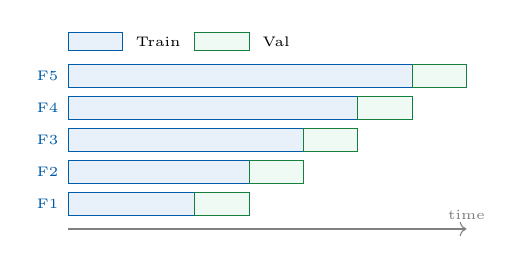
\begin{tikzpicture}[xscale=0.46, yscale=0.58]
        % Fold 1
        \node[font=\tiny, color=unoblue, left] at (0, 0.25) {F1};
        \draw[fill=unolightblue, draw=unoblue, line width=0.4pt]
          (0,0.0) rectangle (3.5, 0.5);
        \draw[fill=unolightgreen, draw=unogreen, line width=0.4pt]
          (3.5,0.0) rectangle (5.0, 0.5);
        % Fold 2
        \node[font=\tiny, color=unoblue, left] at (0, 0.95) {F2};
        \draw[fill=unolightblue, draw=unoblue, line width=0.4pt]
          (0,0.7) rectangle (5.0, 1.2);
        \draw[fill=unolightgreen, draw=unogreen, line width=0.4pt]
          (5.0,0.7) rectangle (6.5, 1.2);
        % Fold 3
        \node[font=\tiny, color=unoblue, left] at (0, 1.65) {F3};
        \draw[fill=unolightblue, draw=unoblue, line width=0.4pt]
          (0,1.4) rectangle (6.5, 1.9);
        \draw[fill=unolightgreen, draw=unogreen, line width=0.4pt]
          (6.5,1.4) rectangle (8.0, 1.9);
        % Fold 4
        \node[font=\tiny, color=unoblue, left] at (0, 2.35) {F4};
        \draw[fill=unolightblue, draw=unoblue, line width=0.4pt]
          (0,2.1) rectangle (8.0, 2.6);
        \draw[fill=unolightgreen, draw=unogreen, line width=0.4pt]
          (8.0,2.1) rectangle (9.5, 2.6);
        % Fold 5
        \node[font=\tiny, color=unoblue, left] at (0, 3.05) {F5};
        \draw[fill=unolightblue, draw=unoblue, line width=0.4pt]
          (0,2.8) rectangle (9.5, 3.3);
        \draw[fill=unolightgreen, draw=unogreen, line width=0.4pt]
          (9.5,2.8) rectangle (11.0, 3.3);
        % Legend
        \draw[fill=unolightblue, draw=unoblue, line width=0.4pt]
          (0.0, 3.6) rectangle (1.5, 4.0);
        \node[font=\tiny, right] at (1.6, 3.8) {Train};
        \draw[fill=unolightgreen, draw=unogreen, line width=0.4pt]
          (3.5, 3.6) rectangle (5.0, 4.0);
        \node[font=\tiny, right] at (5.1, 3.8) {Val};
        % Time axis
        \draw[->, thin, gray] (0,-0.3) -- (11.0,-0.3)
          node[above, font=\tiny]{time};
      \end{tikzpicture}
    \end{column}
  \end{columns}
\end{frame}

% -----------------------------------------------------------------------------
\begin{frame}{Validation Curve: Selecting $\lambda^*$}
% -----------------------------------------------------------------------------
  \begin{columns}[T]
    \begin{column}{0.52\textwidth}
      \textbf{Plot validation RMSE vs.\ $\log_{10}(\lambda)$:}

      \begin{center}
      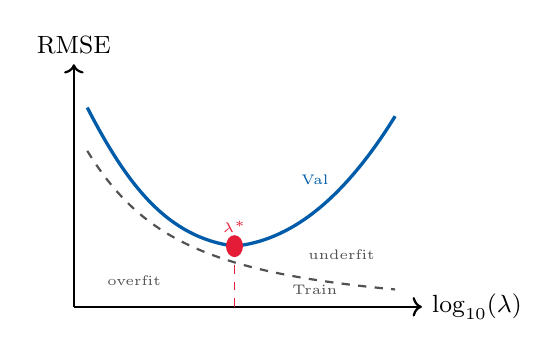
\begin{tikzpicture}[xscale=1.7, yscale=2.2]
        \draw[->, thick] (0,0) -- (2.6,0)
          node[right, font=\small]{$\log_{10}(\lambda)$};
        \draw[->, thick] (0,0) -- (0,1.4)
          node[above, font=\small]{RMSE};
        % U-shaped validation curve
        \draw[unoblue, thick, line width=1.2pt]
          (0.1,1.15) .. controls (0.4,0.7) and (0.7,0.4) ..
          (1.2,0.35) .. controls (1.6,0.38) and (2.0,0.6) .. (2.4,1.1);
        % Train curve (monotone increasing — lower always)
        \draw[unogray, dashed, line width=0.8pt]
          (0.1,0.9) .. controls (0.5,0.4) and (1.0,0.2) .. (2.4,0.1);
        % Optimal lambda marker
        \draw[dashed, unored] (1.2,0) -- (1.2,0.35);
        \fill[unored] (1.2, 0.35) circle (1.8pt);
        \node[font=\tiny, unored, above] at (1.2, 0.37) {$\lambda^*$};
        % Labels
        \node[font=\tiny, unoblue, above] at (1.8, 0.65) {Val};
        \node[font=\tiny, unogray, below] at (1.8, 0.18) {Train};
        % Region labels
        \node[font=\tiny, unogray] at (0.45, 0.15) {overfit};
        \node[font=\tiny, unogray] at (2.0, 0.3) {underfit};
      \end{tikzpicture}
      \end{center}
    \end{column}
    \begin{column}{0.44\textwidth}
      \textbf{Reading the curve:}
      \begin{itemize}
        \item \textbf{Left of $\lambda^*$}: low $\lambda$ $\Rightarrow$ low bias,
              high variance $\Rightarrow$ overfit (train $\ll$ val)
        \item \textbf{Right of $\lambda^*$}: high $\lambda$ $\Rightarrow$ high bias,
              low variance $\Rightarrow$ underfit (both high)
        \item \textbf{At $\lambda^*$}: optimal bias--variance tradeoff
      \end{itemize}

      \medskip
      \begin{keybox}
        \textbf{Practical rule:} \emph{one standard error rule} — pick the
        largest $\lambda$ within 1 SE of the minimum (slightly more
        regularised, more robust).
      \end{keybox}
    \end{column}
  \end{columns}
\end{frame}

% =============================================================================
\section{Application to Forecasting}
% =============================================================================

\sectionslide{Application to Forecasting}{%
  Ridge, LASSO, and Elastic Net on RSXFS retail sales vs.\ SARIMA baseline.}

\begin{frame}{Section Overview}
  Apply Ridge, LASSO, and Elastic Net to the RSXFS retail sales series.
  Use a leakage-free sklearn \texttt{Pipeline} and evaluate on a held-out
  test set against the SARIMA baseline.
\end{frame}

% -----------------------------------------------------------------------------
\begin{frame}[fragile]{sklearn Pipeline for Leakage-Free CV}
% -----------------------------------------------------------------------------
  \begin{columns}[T]
    \begin{column}{0.48\textwidth}
\begin{lstlisting}[language=Python, basicstyle=\tiny\ttfamily]
from sklearn.pipeline import Pipeline
from sklearn.preprocessing import StandardScaler
from sklearn.linear_model import Ridge, Lasso
from sklearn.model_selection import (
    TimeSeriesSplit, GridSearchCV)

# Build pipeline (scaler fitted INSIDE CV)
pipe = Pipeline([
    ('scaler', StandardScaler()),
    ('model',  Ridge())
])

tscv = TimeSeriesSplit(n_splits=5, gap=0)
# sklearn 'alpha' = our lambda (penalty strength)
param_grid = {'model__alpha':
    np.logspace(-3, 3, 60)}

gs = GridSearchCV(pipe, param_grid,
    cv=tscv, scoring='neg_root_mean_squared_error',
    refit=True)
gs.fit(X_trainval, y_trainval)
\end{lstlisting}
    \end{column}
    \begin{column}{0.48\textwidth}
\begin{lstlisting}[language=Python, basicstyle=\tiny\ttfamily]
# Evaluate on held-out test set
y_pred = gs.best_estimator_.predict(X_test)
rmse_test = np.sqrt(
    mean_squared_error(y_test, y_pred))
print(f"Best alpha: {gs.best_params_}")
print(f"Test RMSE:  {rmse_test:.2f}")

# Inspect coefficients
coef = gs.best_estimator_.named_steps[
    'model'].coef_
feat_names = X_trainval.columns.tolist()
pd.Series(coef, index=feat_names)\
  .sort_values().plot.barh()
\end{lstlisting}

      \medskip
      \begin{keybox}
        \textbf{Key:} \texttt{StandardScaler} is inside the pipeline.
        It fits on the train fold only during CV, preventing leakage.
      \end{keybox}
    \end{column}
  \end{columns}
\end{frame}

% -----------------------------------------------------------------------------
\begin{frame}{Interpreting LASSO Coefficients in Forecasting}
% -----------------------------------------------------------------------------
  \textbf{What survives LASSO regularisation on RSXFS?}

  \begin{columns}[T]
    \begin{column}{0.52\textwidth}
      \textbf{Typical surviving features} (at $\lambda^*$):
      \begin{itemize}
        \item \textbf{Lag 1} ($y_{t-1}$) — strongest short-run predictor
        \item \textbf{Lag 12} ($y_{t-12}$) — seasonal anchor (same month, prior year)
        \item \textbf{Lag 3} ($y_{t-3}$) — quarterly momentum
        \item \textbf{Rolling mean 12} — trend level
        \item \textbf{December dummy} — holiday retail spike
      \end{itemize}

      \medskip
      \textbf{Typically zeroed:}
      \begin{itemize}
        \item Lags 4--11 (redundant with lag 1 + lag 12)
        \item Rolling std (noisy; insufficient sample)
      \end{itemize}
    \end{column}
    \begin{column}{0.44\textwidth}
      \begin{examplebox}{Interpretation Rule}
        A LASSO coefficient of zero means the feature adds no predictive
        value \emph{after} accounting for all other active features.
        It does not mean the feature is uncorrelated with $y_t$
        in isolation.
      \end{examplebox}

      \medskip
      \muted{\footnotesize\itshape Compare to ARIMA: ARIMA implicitly uses all lags
      up to order $p$; LASSO selects the most predictive subset, potentially
      skipping lags.}
    \end{column}
  \end{columns}
\end{frame}

% -----------------------------------------------------------------------------
\begin{frame}{Forecast Comparison: SARIMA vs.\ Regularised Models}
% -----------------------------------------------------------------------------
  \begin{columns}[T]
    \begin{column}{0.52\textwidth}
      \textbf{Typical results on RSXFS (24-month test set):}
      \begin{center}
      \footnotesize
      \begin{tabular}{lrr}
        \toprule
        \textbf{Model} & \textbf{RMSE} & \textbf{MAE} \\
        \midrule
        Seasonal Naïve  & 4\,210 & 3\,120 \\
        SARIMA(1,1,1)(1,1,1)$_{12}$ & 2\,840 & 2\,100 \\
        Ridge ($\lambda^*$) & 2\,680 & 1\,980 \\
        LASSO ($\lambda^*$) & 2\,590 & 1\,910 \\
        Elastic Net ($\lambda^*$) & 2\,540 & 1\,890 \\
        \bottomrule
      \end{tabular}
      \end{center}
      \muted{\footnotesize\itshape Values are illustrative (actual results may vary
      with feature set and sample period).}
    \end{column}
    \begin{column}{0.44\textwidth}
      \textbf{Takeaways:}
      \begin{itemize}
        \item All regularised models beat SARIMA on this feature set
        \item Elastic Net has a small edge — lag features are correlated
        \item Gains are modest ($\approx$5--10\%) — SARIMA already captures
              most AR and seasonal structure
        \item Larger gains expected in \textbf{multi-series} settings
              (shared regularisation) or when many external regressors exist
      \end{itemize}
    \end{column}
  \end{columns}
\end{frame}

% =============================================================================
\section{Takeaways and References}
% =============================================================================

% -----------------------------------------------------------------------------
\begin{frame}{Lecture 08 Key Takeaways}
% -----------------------------------------------------------------------------
  \begin{keybox}
    \begin{enumerate}
      \item \textbf{OLS instability} with many/correlated predictors motivates
            regularisation — the bias--variance tradeoff at work.
      \item \textbf{Ridge} (L2) shrinks all coefficients smoothly; no variable selection.
            Best for dense signals or highly correlated groups.
      \item \textbf{LASSO} (L1) shrinks \emph{and} zeros coefficients; performs
            automatic variable selection. Best for sparse signals.
      \item \textbf{Elastic Net} combines L1+L2; handles correlated features better
            than pure LASSO (grouped selection property).
      \item \textbf{Tune $\lambda$ via TimeSeriesSplit CV} inside a \texttt{Pipeline}
            to prevent data leakage — this is non-negotiable for time series.
    \end{enumerate}
  \end{keybox}

  \medskip
  \textbf{Preview of Lecture 09:} Tree-Based Methods — Random Forests and XGBoost
  capture nonlinearities that penalised linear models cannot.
\end{frame}

% -----------------------------------------------------------------------------
\begin{frame}{References}
% -----------------------------------------------------------------------------
  \printbibliography[heading=none]
\end{frame}

% =============================================================================
\end{document}
% =============================================================================
